\chapter{Software-arkitektur}

I følgende afsnit redegøres for det systemets arkitektur og de anvendte patterns sammen med en begrundelse for hvorfor de er valgt.

\section{MVC}
Model-View-Controller\cite{MVC} er et GUI-pattern, der forsøger at adskille den grafiske brugergrænseflade fra resten af systemet. Denne adskillelse har en række af fordele. De væsentligste fordele er, at applikationen bliver mere testbar, skalerbar samt nemmere at vedligeholde. I projektet er der anvendt ASP.NET\cite{ASP} MVC, hvilket er en afart af den rene form for MVC. 
ASP.NET MVC består af tre dele:
\begin{itemize}
	\item Model: er den del der arbejder med den data relaterede logik, dvs. Data Acces Layer. Det er den data der tages fra databasen og bliver manipuleret af Controllers.
	\item View: er den grafiske del af programmet og indeholder præsentationslogikken. Denne del skal være afkoblet fra modellen.
	\item Controller: er grænsefladen mellem modellen og viewet. Controllerens opgave er at manipulere
	data fra modellen og interagere med Views for at vise outputtet og modtage inputs
	fra viewet
\end{itemize}

På  figur  \ref{fig:MVC}  kan  der  ses  den  overordnet  struktur for, hvordan de tre dele af MVC kommunikere indbyrdes.

\begin{figure}[H]
	\centering
	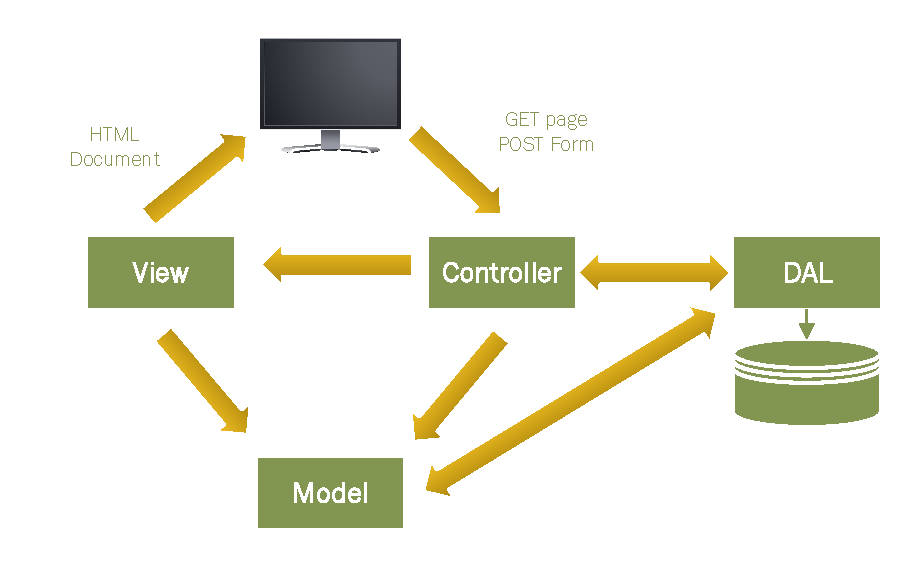
\includegraphics
	[width=140mm]{figures/MVC_drawing.pdf}
	\caption{MVC struktur}
	\label{fig:MVC}
\end{figure}

MVC blev valgt på baggrund af, at det er en integreret del af ASP.NET MVC. ASP.NET MVC er sat op, så applikationens controllere og deres forskellige actions bliver kaldt gennem url'en.
Dette bliver sat op i RouteConfig.cs, hvor der som standard er følgende opsætning:\\
\begin{lstlisting}
    public class RouteConfig
    {
        public static void RegisterRoutes(RouteCollection routes)
        {
            routes.IgnoreRoute("{resource}.axd/{*pathInfo}");

            routes.MapRoute(
                name: "Default",
                url: "{controller}/{action}/{id}",
                defaults: new { controller = "Home", action = "Index", id
                 = UrlParameter.Optional }
            );
        }
    }
\end{lstlisting}
Koden oven over viser, hvordan ASP.NET MVC router mellem de forskellige sider på baggrund af url'en. Det første argument i url'en router til en controller. Det efterfølgende argument er navnet på actionen, der skal kaldes i den valgte controller, hvis dette ikke er angivet kaldes ''Index''-metoden som default. Det sidste sidste argument er parametrene actionen skal kaldes med.
Der er opsat en række af default argumenter, som kaldes, hvis der ikke er angivet nogen. Default argumenterne er følgende:\\
''defaults: new { controller = "Home", action = "Index", id =UrlParameter.Optional }''.

\section{3-lags-modellen}
Systemet bygger på trelags-modellen \cite{3layer}, som kan ses i figur \ref{fig:lagmodel}.
\begin{figure}[H]
	\centering
	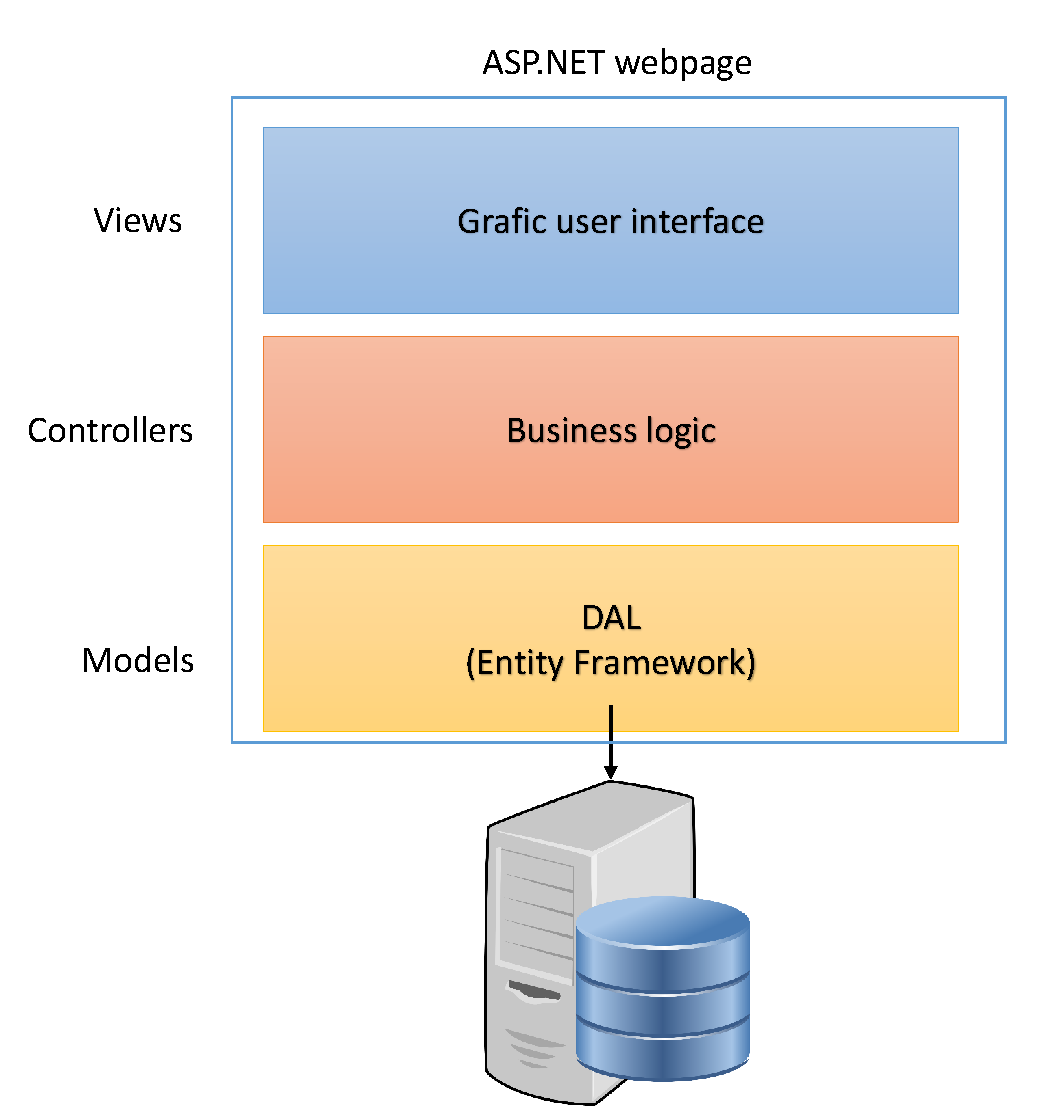
\includegraphics
	[width=165mm]{figures/lagmodel.pdf}
	\caption{Lagmodel for systemet}
	\label{fig:lagmodel}
\end{figure}

3-lags modellen forsøger som MVC at adskille præsentations-, business- og data-access logikken fra hinanden. 3-lags modellen foreskriver, at disse lag skal være fysisk adskilte fra hinanden. Fordelene ved den fysiske adskille basere sig primært på ''separation of concerns'' og ''Single Responsibility'', hvilket medfører et skalerbart og vedligeholdelses venligt system.\\
ASP.NET MVC baseres på 3-lags modellen, hvilket gør, at systemets arkitektur lægger sig tæt op af 3-lags modellen.
Systemets views er præsentationslogikken, controllers og modellen er business-logikken og entity framework samt modellen er systemets Data access lag. 

\subsection{Præsentationslaget}
For web-applikationen generelt, og for de opstillede ikke-funktionelle krav til systemet, er brugervenlighed en væsentlig faktor. Dette betyder at præsentationslogikken er ekstremt vigtig for systemet. Da det skal være let for en bruger at navigere rundt på siden og kunne forstå, hvad meningen er med de forskellige handlinger der kan foretages.

Da projektet er en webapplikation præsenteres den grundlæggende i HTML\cite{HTML} i browseren. HTML'en bliver vha. CSS\cite{CSS} og Javascript\cite{JavaScript} stylet for at opnå et mere overskueligt design. I forbindelse med styling af views er front-end frameworket Bootstrap\cite{Bootstrap} anvendt. Bootstrap er blevet anvendt for at give hjemmesiden et mere responsivt design. Således at hjemmesiden kan benyttes fra flere forskellige typer af enheder (Smartphones, PC mm.), der var et af de ikke-funktionelle krav i afsnit \ref{ch:Ikkefunktionelle}.
Bootstrap er et framework, der arbejder med relative værdier for skærmstørrelsen, således at layoutet skalere og relativt fylder det samme på forskellige typer af enheder/skærmstørrelser.

I  praksis bliver  præsentationslaget i ASP.NET returneret af controllerne til brugeren, der kan se dette i browseren.% Disse controllers foretager en handling med fx et databasekald, hvorefter der returneres et view fra controlleren som brugeren kan se.

\subsection{Businesslag}
Business-laget i projektet er i høj grad controllerne. Der ligger selvfølgelig også nogle forretnings-specifikke valg i modellen. Forretningslogikken ligger derfor som udgangspunkt i controllerne, hvor der er forsøgt at afkoble så meget som muligt af logikken fra præsentationslage. Dette er også er fordel, da controlleren har lettere ved at blive testet i modsætningen til præsentationslaget. I ASP.NET MVC sender man ofte data til viewet fra controlleren som et objekt. Dette gør, at man kan arbejde parallelt på controller og view. Da der i objektet ligger et fast defineret interface. Derfor går en del af forretningslogikken udpå at fremstille eller samle et objekt, der har et klart interface til at kunne blive anvendt i viewet. 

\subsection{Database lag}
I BargainBarter anvendes ADO.NET Entity Framework\cite{ADOEF} som det nederste data access layer. Entity Framework er et framework, der fjerner det impedans mismatch, der ofte opstår mellem databasen og objektmodellen i et projekt. Entity Framework er valgt, da man vha. en objekt orienteret tankegang kan operere på en database. Man slipper derfor for en del bekymringer og ekstraarbejde i form af triviel kode, der skulle skrives i forbindelse med mapningen af database-objekter til kode-objekter. I brugen af Entity Framework har LINQ \cite{LINQ} været et godt hjælpemiddel til at operere på databasen. 

Entity Framework var desuden oplagt, da der i projektet har været stillet en Microsoft SQL Server Database til rådighed af AU. Udover dette arbejder Entity Framework også godt sammen med ASP.Net MVC frameworket.  

I brugen af Entity Framework, anvendes en Code First New Database\cite{EFCodeFirst} approach. På denne måde bliver databasen genereret på baggrund af objektmodellen man opstiller i projektet. Man kan via migrations udvidde objektmodellen og dermed databasen løbende i projektet. Migrations gemmer også historikken over ændringerne på databasen. Dette approach er derfor meget fleksibel, idet man altid kan rulle databasen tilbage til et tidligere stadie. Da man uddelegerer mapningen mellem objektmodellen og entitetsmodellen til et framework, med nogle meget strikse regler kommer disse to forskellige modeller til at ligne hinanden og interfacet fra projektet til databasen bliver derfor meget homogent og let anvendeligt. Gruppen har desuden modtaget undervisning i brug af frameworket i faget I4DAB.

Dette er nogle af grundene til at beslutningen om at anvende Entity Framework. Denne beslutning blev truffet tidligt i projektet, og har i høj grad har indflydelse på arkitekturen for systemet.

\section{Repository Pattern}
Repository pattern er et software mønster \cite{pattern}, der indfører et ekstra lag (Repository-lag) mellem databasen og buisness-logikken. Det virker som data-access lag mellem buisness-logikken og det oprindelige data-access lag - i dette tilfælde Entity Framework. Dette ekstra lag medfører, at buisness-logikken ikke skriver direkte ned i databasen. Dette sænker i høj grad koblingen i systemet, da buisness-laget ikke er afhængig af databasen. 
Buisness-laget kalder bare ned i repository-laget, der så sørger for selve transaktionen med databasen. 
På figur \ref{fig:Repository} kan man se, hvor og hvordan det ekstra lag indføres i arkitekturen.

\begin{figure}[H]
	\centering
	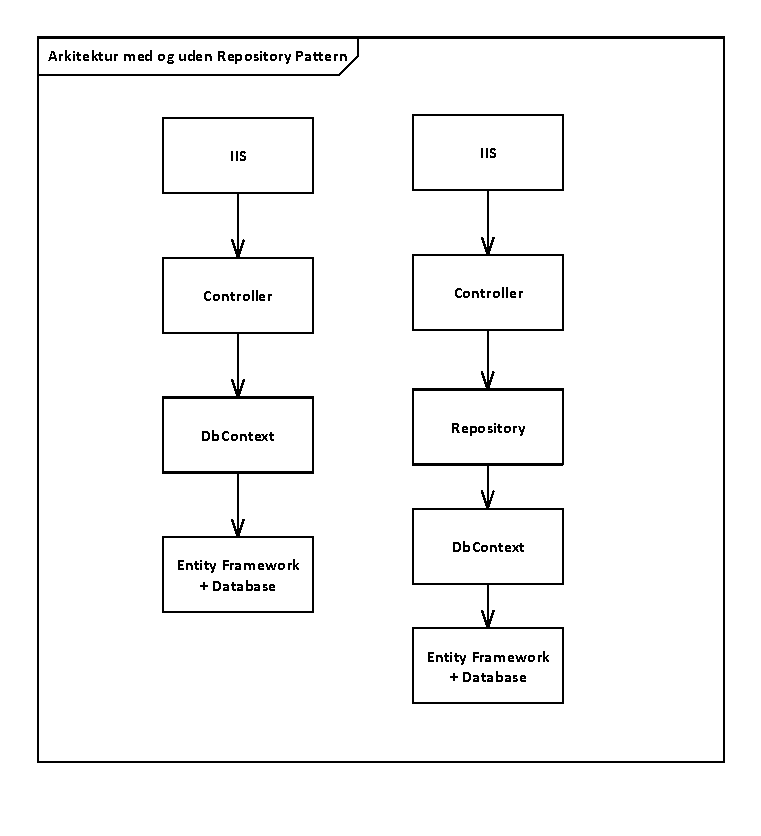
\includegraphics
	[width=140mm]{figures/Repository1.pdf}
	\caption{Respository Patterns betydning for arkitekturen}
	\label{fig:Repository}
\end{figure}

Repository pattern er blevet anvendt for at opnå en lavere kobling i systemet mellem databasen og buisness-logikken. Den lavere kobling i systemet, gør systemet mere robust for ændringer. Systemet bliver også samtidig mere testbart, da det på denne måde kan benytte despendency inversion, hvor ved de forskellige database afhængigheder kan mockes ud i forbindelse med testningen af systemet. 

\section{Unit Of Work}
Unit of Work er et design pattern, der holder styr på in-memory opdateringer og skriver disse opdateringer til databasen. Dette er dermed den eneste klasse, der taler sammen med databasen.
Dette er blevet opnået ved at, at Unit Of Work-klassen indeholder en række GenericRepository's af alle de forskellige model-klasser. Det er Unit Of Work, der vedligeholder disse repositories. Unit Of Work er den eneste, der tilføjer eller sletter i databasen. Det er dermed Unit Of Work, der laver de gængse database-transaktioner og sørge for at databasen bliver opdateret, når en transaktion er afsluttet.

\section{Valg af Teknologier}
\subsection{ASP.NET}
ASP.NET er et udviklings framework for web-applikationer.
Det er en del af .NET Frameworket, der gør at al kode, der er  kompatible med .NET og CLR også er kompatibelt i ASP.NET. Dette har været en af de væsentligste grunde til, at ASP.NET er blevet benyttet, da det har gjort at projektet kunne skrives i C\#, der er blevet undervist i på semesterets andre kurser. Gruppen har desuden også modtaget undervisning i ASP.NET i forbindelse med faget I4GUI.

\subsection{SignalR}
SignalR\cite{SignalR} er et software-biblotek til ASP.NET miljøet. Biblioteket giver adgang til at benytte real-time funktioner på det website man udvikler på. Det kan benyttes, når man vil have en form for interaktion med brugerne, eller mellem brugere. \\
Det forgår i browseren ved brug af javascript-kode, men der kan stadig laves kald tilbage til serveren. 
SignalR er blevet anvendt for til at implementere systemets real-time chat.

\section{Generelle overvejelser i forbindelse med Arkitektur}
I forbindelse med projektet har der været nogle generelle overvejelser, omkring den arkitektur produktet skulle have. Et af de vigtigste key issues har været brugerkvaliteten. Dvs. at brugervenligheden og skalerbarheden til forskellige apparater, har skullet være i top for at produktet har kunne give værdi. Dette er kommet til livs med at anvende frameworket Bootstrap, som er en stor hjælp til at lave pæne designs, der skalerer til forskellige devicestørrelser, uden alt for meget arbejde. 

Et andet kriterie der er tænkt ind i arkitekturen er performance. Dette kan bl.a. ses ved implementeringen af chatten. I chat controlleren er meget af logikken implementeret client side vha. javascript. Dette giver en bedre brugeroplevelse da opdateringerne sker øjeblikkeligt i chatten, da der kan spares nogle kald til serveren.

Af cross cutting concerns i projektet har der bl.a. været verificering af en brugers log-in på de forskellige sider. Dvs. at visse dele af hjemmesiden ikke skulle være tilgængelig, med mindre brugeren var logget ind. Til at løse dette problem er ASP.NET identity\cite{Identity} blevet brugt og udvidet, med de oplysninger der har været nødvendige for at projektet har passet på domænet.

En anden cross cutting concern er validering af oplysninger når en brugerprofil oprettes. I projektet er det valgt at brugeren skal oplyse en adresse, fulde navn, email, password og telefonnummer. Adresse og kontaktinformationer er valgt, da disse oplysninger alle er essentielle for at en byttehandel kan finde sted i virkeligheden. Passwordet er valgt til ikke at have særligt strikse krav, idet oplysningerne ikke er særligt kritiske at miste. Det er derfor vigtigere at brugerens indgangsbarriere er minimal, og at der ikke at skulle bruges for lang tid på at finde på et password, som han/hun alligevel ikke kan huske bagefter.